The Low Level Abstract Machine~(LLAM) implements the complete operational
semantics of LM and builds on top of HLD by turning all the non-deterministic
choices of HLD into deterministic steps. LLAM specifies the following:

\begin{itemize}

   \item Rule matching by priority order;

   \item Deterministic matching of rule, comprehension and
      aggregate bodies;

   \item Iteration over all available combinations of facts for comprehensions/aggregates.

\end{itemize}

While HLD was represented as a proof tree with multiple choices, LLAM is defined
as a sequence of state transitions of the form $\trans{S_1}{S_2}$.  The LLAM
presents a complete step by step mechanism that is needed to correctly evaluate
an LM program. For instance, when LLAM tries to apply a rule, it checks if there
are enough facts in the database and backtrack until some rule can be inferred.

\paragraph{Continuation Stack} The core idea of LLAM is the \emph{continuation
stack}. A continuation stack contains \emph{continuation frames} that are
created for each predicate needed from the database. For instance, the first
rule in Fig.~\ref{code:visit} needs 3 frames: \code{visit}, \code{visited} and
\code{edge}. A frame allows the LLAM to search over facts of a given predicate
in order to match terms and thus contains candidate facts that will be
attempted. Each frame stores the contexts required to restart the matching
process. We have \emph{linear} and \emph{persistent frames}, which are created
for linear and persistent fact expressions, respectively.  We discuss only
linear frames, which have the form $\lframe{\Delta}{\Delta''}{p}{\Omega;
\Psi}{\Delta'}{\Omega'}$, where:

\begin{enumerate}

  \item[$\Delta$] multi-set of linear facts that are not of predicate $p$ plus
all the other $p$'s we have tried already, including the current $p$;

  \item[$\Delta''$] all the other $p$ facts we have not tried yet. It is a multi-set
  of linear facts;

  \item[$p$] fact expression that created this frame;

  \item[$\Omega$] ordered list of remaining terms needed to match past this
  frame;

  \item[$\Delta'$] multi-set of linear facts we have consumed to reach this
     point in the process;

  \item[$\Omega'$] terms matched up-to this point using $\Delta'$ and $\Gamma$. 
The frame proposition $\mz{\Gamma}{\Delta'}{\Omega'}$ represents a valid HLD
matching proposition. This will be used during the soundness proof in the next
section.

   \item[$\Psi$] current variable assignments (includes variable and value).
     
\end{enumerate}

\paragraph{Matching} For a rule of the form $\forall_{\widehat{x}}. A \lolli B$,
matching starts with an empty continuation stack and term $A$ has a term to
match that contains the (now) free variables $\widehat{x}$ that need to be
matched, as show in the following LLAM state:

\vspace{-3mm}
\[
   \matstate{A \lolli B}{(\Delta; \Phi)}{\cdot}{\Gamma}{\Delta}{A}{\cdot
   \rightarrow \one}
\]
\vspace{-3mm}

No shown in the matching state is the context $\Psi$ that maps variables to
values. At the start of matching, the $\widehat{x}$ variables are set as
\emph{undefined}. The terms to match are then deconstructed in an ordered
context and continuation frames are pushed onto the stack whenever a new fact
appears in the body. New facts also update the variables in the $\Psi$ contexts
by assigning them concrete values. Like the frames shown before, each matching
state also contains a proposition $\mz{\Gamma}{\Delta'}{\Omega'}$ that is an HLD
proof built by de-constructing and matching terms.

The following transitions model linear expression matching. $p_1, \Delta'' \prec
p$ means that the database facts $p_1, \Delta''$ satisfy the constraints of
$p$\footnote{Constraints such as variable matchings using the current $\Psi$
context.} by using the omitted variable context $\Psi$. The context $\Delta''$
is pushed into the new continuation frame because it is the set of candidate
facts to try next.

\vspace{-5mm}
\[
\infer[\mo p~\m{first}]
{\mo \Gamma ; \Delta, p_1, \Delta'' ; \Xi; p, \Omega; H; \cdot; \lstack{R} \rightarrow
   \outsem}
{
 \begin{gathered}
   p_1, \Delta'' \prec p \\
   \mo \Gamma ; \Delta, \Delta''; \Xi, p_1; \Omega; H;
      (\Delta, p_1; \Delta''; p; \Omega; \Xi; \cdot; \cdot); \lstack{R} \rightarrow
      \outsem
  \end{gathered}
}
\]

\[
\infer[\mo p~\m{on}~q]
{\mo \Gamma ; \Delta, p_1, \Delta'' ; \Xi; p, \Omega; H; f, \lstack{C};
   \lstack{R} \rightarrow \outsem}
{
\begin{gathered}
   p_1, \Delta'' \prec p \\
   f = (\Delta_{old}; \Delta'_{old}; q; \Omega_{old}; \Xi_{old}; \Lambda;
         \Upsilon) \\
   \mo \Gamma ; \Delta, \Delta''; \Xi, p_1; \Omega; H; (\Delta, p_1; \Delta'';
         p; \Omega; \Xi; q, \Lambda; \Upsilon), f, \lstack{C}; \lstack{R} \rightarrow \outsem
\end{gathered}
}
\]


\[
\infer[\mo p~\m{on}~\bang q]
{\mo \Gamma ; \Delta, p_1, \Delta'' ; \Xi; p, \Omega; H; f, \lstack{C};
   \lstack{R} \rightarrow \outsem}
{
\begin{gathered}
   p_1, \Delta'' \prec p \\
   f = [\Gamma_{old}; \Delta_{old}; \bang q; \Omega_{old}; \Xi_{old}; \Lambda; \Upsilon] \\
   \mo \Gamma ; \Delta, \Delta''; \Xi, p_1; \Omega; H; (\Delta, p_1; \Delta''; p; \Omega; \Xi;
         \Lambda; q, \Upsilon), f, \lstack{C}; \lstack{R} \rightarrow \outsem
\end{gathered}}
\]

\[
\infer[\mo p~\m{fail}]
{\mo \Gamma ; \Delta; \Xi; p, \Omega; H; \lstack{C}; \lstack{R} \rightarrow \outsem}
{\Delta \npreceq p & \cont \lstack{C} ; H; \lstack{R}; \Gamma \rightarrow \outsem}
\]

\vspace{-5mm}

LLAM also uses a special \emph{rule continuation stack} represented as $\rulestk
= (\Delta; \Phi)$ that tries all the rules in order. This fulfills the semantics
of LM for deriving the highest priority rule. In terms of inputs and outputs,
LLAM is equal to HLD.

\paragraph{Continuation} If, during the matching process, the machine is unable
to retrieve candidate facts for a given fact using $\Psi$, it backtracks to try
other facts in order to use different variable assignments in $\Psi$. The top
frame of the continuation stack is updated to retrieve the next candidate fact
and then restore the matching process using the frame's contexts.

The following two transitions model LLAM continuation states. In the first
transition, the next candidate fact is retrieved from the linear frame and the
linear frame is updated. In the second transition, since there is no candidate,
the frame is thrown away and the next frame is used.

\vspace{-5mm}
\[
\infer[\cont p~\m{next}]
{\cont (\Delta; p_1, \Delta''; p, \Omega; \Xi; \Lambda; \Upsilon), \lstack{C};
   H; \lstack{R}; \Gamma \rightarrow \outsem}
{\mo \Gamma ; \Delta, \Delta''; \Xi, p_1; \Omega; H; (\Delta, p_1; \Delta''; p,
      \Omega; H; \Xi; \Lambda; \Upsilon), \lstack{C}; \lstack{R} \rightarrow \outsem}
\]

\[
\infer[\cont p~\m{no~more}]
{\cont (\Delta; \cdot; p, \Omega; \Xi; \Lambda; \Upsilon), \lstack{C}; H;
   \lstack{R}; \Gamma
   \rightarrow \outsem}
{\cont \lstack{C}; H; \lstack{R}; \Gamma \rightarrow \outsem}
\]

\vspace{-5mm}

\paragraph{Derivation}

Once matching completes, the terms are derived by de-constructing the head terms
into an ordered context. Next, the terms are derived sequentially, including
comprehensions and aggregates. The following rule shows the transition from a
derivation state to the final state of the machine:

\vspace{-5mm}
\[
\infer[\done \m{end}]
{\done \Gamma; \Delta; \Xi; \Gamma_1; \Delta_1; \cdot \rightarrow \Xi; \Gamma_1;
\Delta_1}
{}
\]

\vspace{-5mm}

The contexts $\Gamma_1$ and $\Delta_1$ contain facts that were derived from head
terms.

\paragraph{Aggregates}

Both aggregates and comprehensions use the same matching and continuation
mechanism shown before.  Consider an aggregate of the form
$\aggregate{\mathtt{cons ::}}{\sigma}{\widehat{x}}{A}{B}{C}$. We start with an
empty continuation stack and match $A$.  The LLAM transition for initializing
the computation of aggregates is as follows:

\vspace{-5mm}
\[
\infer[\done \m{agg}]
{\done \Gamma; \Delta ; \Xi; \Gamma_1; \Delta_1; \aggsz{A}{B}{C}, \Omega
   \rightarrow \outsem}
{\ma \Gamma; \Delta; \Xi; \Gamma_1; \Delta_1; \cdot; A ; \cdot; \cdot;
   \aggsz{A}{B}{C}; \Omega; \Delta; \cdot \rightarrow \outsem}
\]

\vspace{-4mm}

If matching is successful then the first application of the aggregate is
completed and $B$ is derived for that particular combination.  At this point,
the aggregate value is saved in the judgment to be aggregated later with all the
remaining values\footnote{Since the aggregate references an accumulator variable
$\sigma$, we use $\Psi(\sigma)$ to retrieve the value.}.

The semantics of aggregates require all the combinations of $A$ from
the database. We reuse the continuation stack created by the first
application. All the frames after the first continuation frame for a linear fact
need to be removed and then the remaining frames need to be updated in order to
delete the consumed facts from the contexts. For example, if the body $A$ is
$\mathtt{b(X)} \otimes \mathtt{c(X)} \otimes \mathtt{b(Y)}$ and the continuation
stack has three frames (one per fact), we cannot backtrack to the frame of
$\mathtt{b(Y)}$ because, at that point, the matching process was assuming that
the previous $\mathtt{c(X)}$ linear fact was still available.  Moreover, we also
need to remove the consumed linear facts from the $\mathtt{b(X)}$ frame
since the candidate context may contain a $\mathtt{b}$ fact that was deleted
for $\mathtt{b(Y)}$. Note that we use two separate continuations in order to
mark the offset in the stack where the first linear continuation frame was
pushed.

The aggregate computation continues by restarting the matching process at the
top of the continuation stack and then matching the body of the aggregate once
again. This repeated process eventually iterates over the database. The
aggregate completes when the continuation stack is exhausted. The final
aggregate head $C$ is then derived with the aggregated value $\Sigma$ as shown
in the transition below:

\vspace{-5mm}
\[
\infer[\conta{\aggsz{A}{B}{C}} \m{end}]
{\conta{\aggsz{A}{B}{C}} \Gamma; \Delta_N; \Xi_N; \Gamma_{N1}; \Delta_{N1}; \cdot; \cdot;
   \Omega; \Sigma \rightarrow \outsem}
{\done \Gamma; \Delta_N; \Xi_N; \Gamma_{N1}; \Delta_{N1}; (\lambda x. C
      x)\Sigma,
   \Omega \rightarrow \outsem}
\]

\vspace{-4mm}

Figure~\ref{fig:backtrack} shows how the aggregate in the pagerank code shown in
Fig.~\ref{code:pagerank} is computed. Let's assume that \code{A = 1} and that
there are four facts: \code{edge(1,2)}, \code{edge(1,3)},
\code{pagerank(2,0.5)}, \code{pagerank(3,0.5)}. An initial frame is created for
\code{edge(1,B)} which includes two \code{edge} facts and \code{edge(1,2)} is
selected to continue the process.  Since \code{B = 2}, the frame for
\code{pagerank} includes only \code{pagerank(2,0.5)} which completes the first
application of the aggregate and every linear fact used is re-derived using the
first aggregate head. Computation then proceeds by backtracking to the first
linear frame, namely, the frame of \code{edge(1,B)} and the \code{edge(1,3)} is
selected for matching. A frame for \code{pagerank(3,V)} is created and the
second application of the aggregate re-derives the head. For the third
application, we backtrack again to the first linear frame, but there are no
available candidates and no more frames and thus the second aggregate head is
derived using \code{V = 0.5 + 0.5} as the result, completing the aggregate.

\begin{figure}[ht]
   \begin{center}
      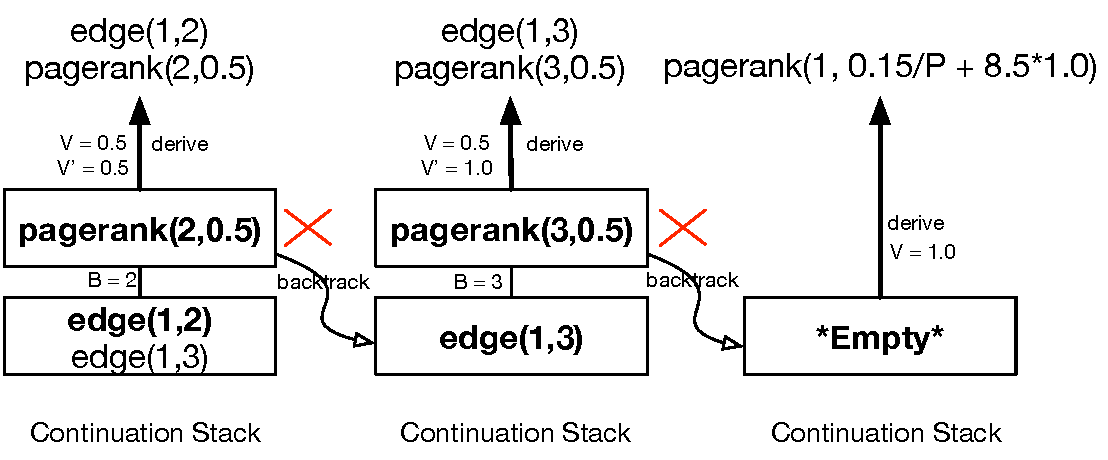
\includegraphics[width=0.7\linewidth]{figures/backtrack.pdf}
   \end{center}
   \caption{Generating the pagerank aggregate.}
   \label{fig:backtrack}
   \vspace{-5mm}
\end{figure}
